
\documentclass{abgabe}
\begin{document}

\begin{questions}
    \qformat{\thequestion. \textbf{\thequestiontitle} \hfill}
    \titledquestion{Aktivitätsdiagramm Pfannkuchenrezept}

    Gegeben ist das unten angegebene Rezept.
    Stellen Sie den Vorgang der Zubereitung eines Pfannkuchens in Form eines \emph{Aktivitätsdiagramms} z.B. mit Hilfe von \href{https://www.ili.fh-aachen.de/ilias.php?baseClass=ilLinkResourceHandlerGUI&ref_id=341847&cmd=calldirectlink}{Visual Paradigm} dar!

    Berücksichtigen Sie dabei möglichst \emph{alle} Details des Rezeptes sowie die im Prozess entstehenden Objekte! Überlegen Sie auch, welche Aktionen parallel stattfinden können!

    {\large Zutaten}\footnotemark
    \begin{itemize}
        \item 4 TL Ei-Ersatzpulver
        \item 8 EL Wasser
        \item Mehl
        \item Pflanzenmilch
        \item 1 Apfel
        \item veganer Wurst-/Käseersatz
        \item Marmelade
        \item Apfelmus
        \item Zucker
    \end{itemize}

    {\large Zubereitung}
    \begin{itemize}
        \item Ei-Ersatzpulver und Wasser in einer Schüssel vermengen
        \item solange Mehl hinzugeben, bis Teig schwer zu rühren ist
        \item solange Pflanzenmilch hinzugeben, bis die Masse wieder leicht zu rühren ist, damit sie sich gut in der Pfanne verteilen lässt
        \item etwas Pflanzenmargarine in einer Pfanne erhitzen
        \item Teil der Masse in die Mitte der Pfanne geben, bis der Boden bedeckt ist
        \item bei der süßen Variante können Apfelscheiben dazu gegeben werden - bei der herzhaften Variante Wurst- und Käseersatz
        \item die Pfannkuchen von beiden Seiten gut anbraten
        \item die süßen Pfannkuchen können nach Belieben, z.B. mit Marmelade, Apfelmus oder Zucker garniert werden
    \end{itemize}

    \footnotetext{Das Rezept ist beabsichtigt leicht verändert. Reddit-User \href{https://www.reddit.com/r/vegan/comments/a2936b/why_you_should_go_vegan_ultimate_facts_and/}{Sbeast} fasst es sehr gut zusammen.}

    \clearpage
    \begin{solution}
        \begin{center}
            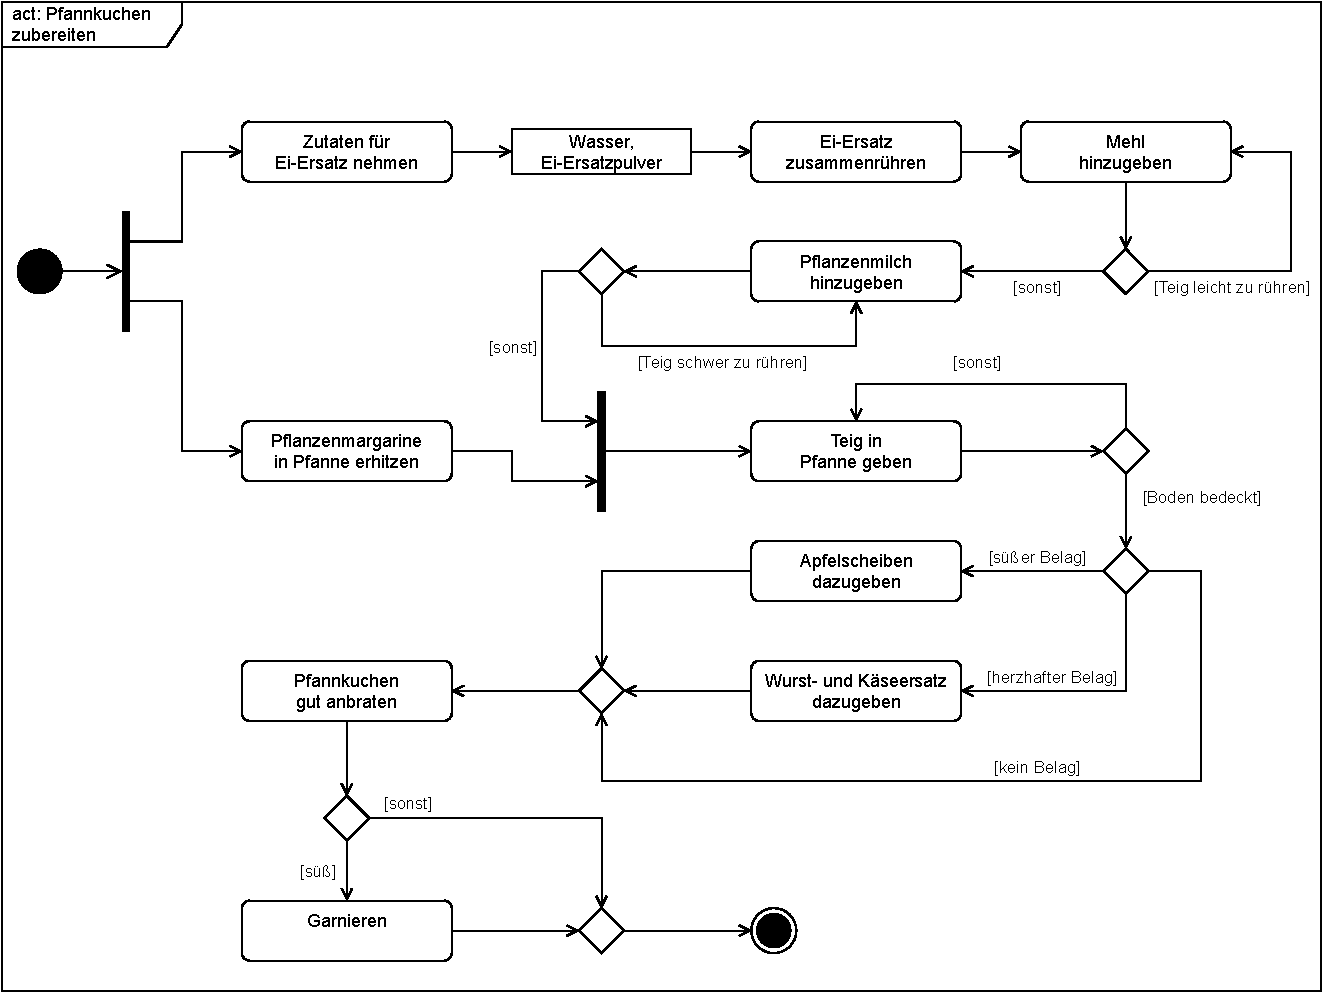
\includegraphics[width=\textwidth]{swt_h05_pfannkuchen.pdf}
        \end{center}
    \end{solution}
\end{questions}
\end{document}